\section{Detekcja}



\subsection{Wnioski}

\section{Dane treningowe}
Za dane wejściowe do procesu trenowania sieci neuronowych wybrano \fnurl{Glasgow Unfamiliar Face Database (GUFD)}{http://www.facevar.com/glasgow-unfamiliar-face-database}, która dostępna jest za darmo i można jej używać na potrzeby badań uczelnianych oraz publikacji. Jedynym warunkiem użycia jest zacytowanie jednej z publikacji właściciela bazy.

Baza zawiera 303 tożsamości. Na każdą z tożsamości składa się 20 zdjęć jednej osoby wykonanych w różnych warunkach np. różniące się kąty ujęcia, wyrazy twarzy oraz z dodatkowymi akcesoriami(okulary, kaptur, czapka). 

\section{Trenowanie sieci neuronowych}
Podczas badania sieci neuronowych postanowiono sprawdzić kilka podstawowych czynników, na które składa się wpływ ilości wybranych tożsamości oraz wpływ ilości zdjęć przydzielonych tożsamości na:
\begin{itemize}
\item czas potrzebny na preprocessing danych uczących,
\item czas trwania trenowania modelu,
\item rozmiar pliku zawierającego model (jeśli istnieje).
\end{itemize}
W rozdziale \ref{b:rozpoznawanie} omówiono wpływ wyżej wymienionych parametrów na czas oraz pewność identyfikowania tożsamości.

\begin{figure}[H]
	\centering
	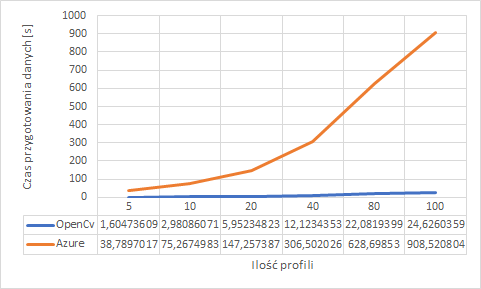
\includegraphics[scale=1.0]{czas_przygotowania_a_ilosc_profili.png}
	\caption{Schemat klasycznego wzorca MVC}
	\label{fig:schemat_mvc}
\end{figure}

\begin{figure}[H]
	\centering
	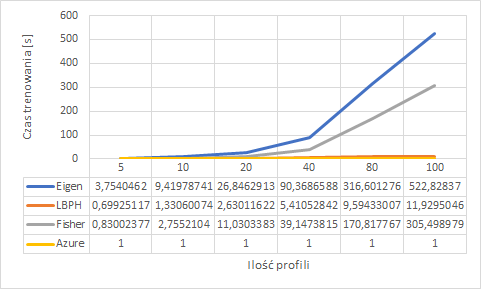
\includegraphics[scale=1.0]{czas_trenowania_a_ilosc_profili.png}
	\caption{Schemat klasycznego wzorca MVC}
	\label{fig:schemat_mvc}
\end{figure}

\begin{figure}[H]
	\centering
	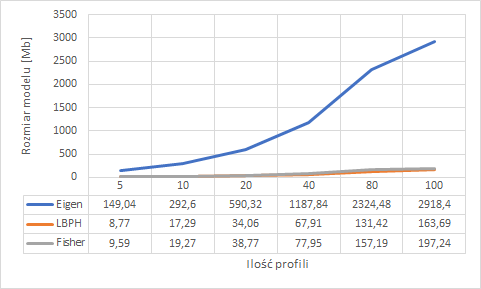
\includegraphics[scale=1.0]{rozmiar_modelu_a_ilosc_profili.png}
	\caption{Schemat klasycznego wzorca MVC}
	\label{fig:schemat_mvc}
\end{figure}

\begin{figure}[H]
	\centering
	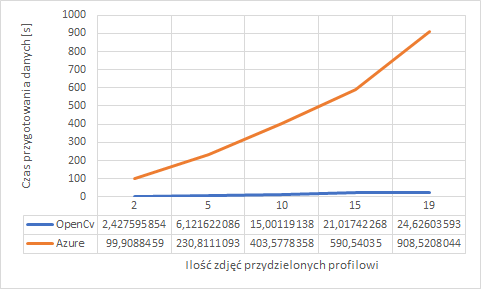
\includegraphics[scale=1.0]{czas_przygotowania_a_ilosc_zdjec.png}
	\caption{Schemat klasycznego wzorca MVC}
	\label{fig:schemat_mvc}
\end{figure}

\begin{figure}[H]
	\centering
	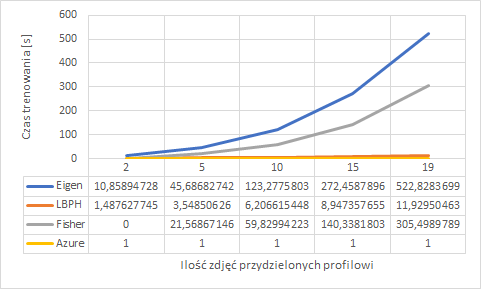
\includegraphics[scale=1.0]{czas_trenowania_a_ilosc_zdjec.png}
	\caption{Schemat klasycznego wzorca MVC}
	\label{fig:schemat_mvc}
\end{figure}

\begin{figure}[H]
	\centering
	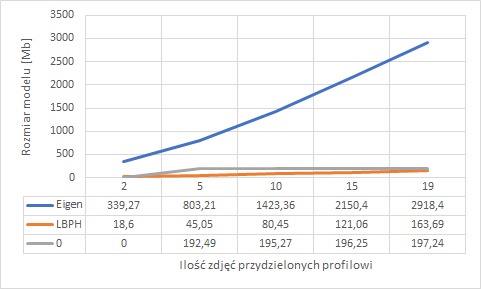
\includegraphics[scale=1.0]{rozmiar_modelu_a_ilosc_zdjec.png}
	\caption{Schemat klasycznego wzorca MVC}
	\label{fig:schemat_mvc}
\end{figure}

\subsection{Wpływ ilości próbek na czas tworzenia modelu}
kilka testów
\subsection{Wpływ ilości próbek na rozmiar modelu}
kilka testów

\section{Rozpoznawanie twarzy} \label{b:rozpoznawanie}
\subsection{Wpływ ilości próbek na pewność rozpoznania}

\subsection{Porównanie wyników}
\subsection{Czas przetwarzania zapytania}

\section{Ocena przydatności wybranych usług IoT}



Konfiguracja bazy danych oraz maszyny wirtualnej okazała się równie prosta w każdym ze środowisk. Proces konfiguracji odbywał się poprzez wypełnienie kilku formularzy niewymagających wprowadzania dużej ilości informacji (ze względu na ograniczenia studenckiej licencji). Na końcu procesu uzyskany zostaje connection string oraz konto za pomocą, którego można zalogować się na serwer.

Największa różnica między dwoma dostawcami wystąpiła w przypadku usług hostujących aplikację webową czyli Azure App Service oraz AWS Elastic Beanstalk. Podczas pierwszych testów konfiguracji aplikacja internetowa istniała jedynie w rozwiązaniu przygotowanym w języku Angular 4. Struktura aplikacji została przygotowana na podstawie wzoru przygotowanego przez Microsoft. Azure App Service bezproblemowo wspierał nawet najnowsze wersje rozwiązań przygotowanych dla .NET Core 2. Niestety AWS nie był przygotowany 